\begin{wrapfigure}{l}{0.45\textwidth}
  \scalebox{0.9}{
    \hspace{-8pt}
    \begin{tabular}{m{1pt}c}
      \multirow{2}*{
        \rotatebox{90}{\tiny magnitude $w_i$}
      }
      \hspace{2pt}
      &
      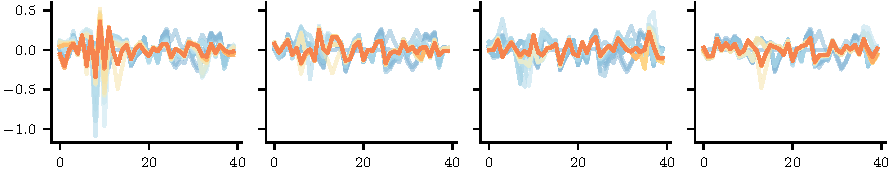
\includegraphics[width=\linewidth]{figures/multi-neuron/10erf_alg4_subset4.pdf} \\ 
      &
      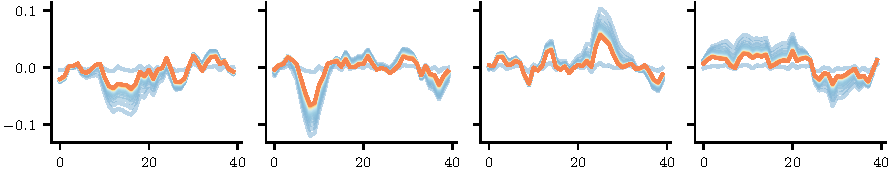
\includegraphics[width=\linewidth]{figures/multi-neuron/10erf_alg30_subset4.pdf}  \\
      \noalign{\vskip -4pt}
      &\hspace{18pt}\tiny dimension $i$ of weight $\mathbf{w}$
    \end{tabular}
  }
  \caption{
    Receptive fields learned by the many-neuron model (\labelcref{item:many-neuron-model})
    with learnable second-layer weights, $N=40$, $K=10$.
    (\textbf{Top}) A random subset of 4 receptive fields from a model with sigmoid activation, 
    trained on $\texttt{Kur(4)}$ (positive excess kurtosis of $3.28$).
    As predicted by Claim~\labelcref{thm:localization},
    the receptive fields are \emph{not} localized, and appear as high-frequency oscillations.
    (\textbf{Bottom}) A random subset of 4 receptive fields from a model with ReLU activation,
    trained on $\texttt{Kur(30)}$ (negative excess kurtosis of $-1.17$).
    Receptive fields are localized (\textbf{left three}) or exhibit low-frequency oscillations (\textbf{right}).
    \emph{See \cref{sec:extensions} for exposition.} 
  }
  \label{fig:multi-neuron}
\end{wrapfigure}
